\documentclass[whitelogo]{tudelft-report}
\usepackage{natbib}
\usepackage{changes}
\usepackage{multirow}
\usepackage{longtable,supertabular,booktabs}


\providecommand{\tightlist}{%
  \setlength{\itemsep}{0pt}\setlength{\parskip}{0pt}}

\usepackage{graphicx,grffile}
\makeatletter
\def\maxwidth{\ifdim\Gin@nat@width>\linewidth\linewidth\else\Gin@nat@width\fi}
\def\maxheight{\ifdim\Gin@nat@height>\textheight\textheight\else\Gin@nat@height\fi}
\makeatother
% Scale images if necessary, so that they will not overflow the page
% margins by default, and it is still possible to overwrite the defaults
% using explicit options in \includegraphics[width, height, ...]{}
\setkeys{Gin}{width=1.0\maxwidth,height=0.4\maxheight,keepaspectratio}

\begin{document}

%% Use Roman numerals for the page numbers of the title pages and table of
%% contents.
\frontmatter

\title[tudelft-white]{EuroToken}
\subtitle[tudelft-black]{A Stable Digital Euro Based on TrustChain}

\author[tudelft-white]{R. W. Blokzijl}
\affiliation{Technische Universiteit Delft}
\coverimage{tank.jpg}

\covertext[tudelft-white]{
    % \textbf{Keywords} \\
	    	- Stablecoin \\
	    	- Blockchain \\
	    	- Cryptocurrencies \\
	    	- TrustChain \\
	    	- CBDC \\
	    \vfill
			R.W.Blokzijl@student.tudelft.nl
	}
\setpagecolor{tudelft-cyan}
\makecover[split]


%% Include an optional title page.
\begin{titlepage}

\begin{center}

%% Insert the TU Delft logo at the bottom of the page.

%% Print the title in cyan.
{\makeatletter
\largetitlestyle\fontsize{64}{94}\selectfont\@title
%\largetitlestyle\color{tudelft-cyan}\Huge\@title
\makeatother}

%% Print the optional subtitle in black.
{\makeatletter
\ifx\@subtitle\undefined\else
    \bigskip
   {\tudsffamily\fontsize{22}{32}\selectfont\@subtitle}
    %\titlefont\titleshape\LARGE\@subtitle
\fi
\makeatother}

\bigskip
\bigskip

by
%door

\bigskip
\bigskip

%% Print the name of the author.
{\makeatletter
%\largetitlefont\Large\bfseries\@author
\largetitlestyle\fontsize{26}{26}\selectfont\@author
\makeatother}

\bigskip
\bigskip

to obtain the degree of Master of Science
%ter verkrijging van de graad van Master of Science

at the Delft University of Technology,
%aan de Technische Universiteit Delft,

to be defended publicly on TODO.
%in het openbaar de verdedigen op dinsdag 1 januari om 10:00 uur.

\vfill

\begin{tabular}{lll}

	    Student number: & 4269519 \\
    	    Project duration: & \multicolumn{2}{l}{November 11, 2020 -- TODO} \\
    	    Thesis committee:
		    	& Dr.ir. J.A. Pouwelse, & TU Delft, supervisor \\
    	    	& Member 1, & TU Delft \\
    	    	& Member 2, & TU Delft \\
    	    \end{tabular}
%% Only include the following lines if confidentiality is applicable.

\bigskip
\bigskip
\emph{This thesis is confidential and cannot be made public until TODO.}
%\emph{Op dit verslag is geheimhouding van toepassing tot en met 31 december 2013.}

\bigskip
\bigskip
An electronic version of this thesis is available at \url{http://repository.tudelft.nl/}.
%\\[1cm]

%\centering{
\includegraphics{cover/logo_black}}


\end{center}

\begin{tikzpicture}[remember picture, overlay]
    \node at (current page.south)[anchor=south,inner sep=0pt]{
        
\includegraphics{cover/logo_black}
    };
\end{tikzpicture}

\end{titlepage}

\chapter*{Preface}
\setheader{Preface}

TODO: Add preface

\begin{flushright}
{\makeatletter\itshape
    \@author \\
    Delft, TODO
\makeatother}
\end{flushright}


\tableofcontents

%% Use Arabic numerals for the page numbers of the chapters.
\mainmatter

\chapter{Introduction}\label{introduction}

\begin{itemize}
\tightlist
\item
  Physical money is slow - restricted by the speed of travel
\item
  Digital money is less slow - restricted by the speed of human
  communication
\item
  New digital money - restricted by the speed of light (and the runtime
  of cryptographic algorithms)
\end{itemize}

\chapter{Problem description}\label{problem-description}

We formulate the problem description as follows:

\begin{longtable}[]{@{}l@{}}
\toprule
\begin{minipage}[t]{0.97\columnwidth}\raggedright\strut
The euro zone is missing an option for a digital currency that mirrors
all features of the euro, while providing the benefits of distributed
accounting and programmable money.\strut
\end{minipage}\tabularnewline
\bottomrule
\end{longtable}

In the historic paper ``On the Origin of Money'' ({\textbf{???}}) Karl
Menger describes how people settle on a currency as a method of
exchange. He describes that the willingness of people to exchange their
goods for a commodity depends upon:

\begin{enumerate}
\def\labelenumi{\arabic{enumi}.}
\tightlist
\item
  The ability to trade the currency for goods and services
\item
  The scarcity of the commodity
\item
  The uniformity, divisibility, durability and practicality of the
  commodity.
\item
  The development of the market, and how others speculate.
\item
  The limitations imposed politically and socially upon exchange,
  consumption and transfer from one period of time to another
\end{enumerate}

All these aspects must be managed in any successful currency. In this
chapter we will work out these requirements into a concrete set of
requirements for the EuroToken system.

\section{The general requirements for
money}\label{the-general-requirements-for-money}

Points 1 and 4, the future usefulness of the currency and it's market
demand, are where digital currencies still fall short of traditional
currencies. Because of the price volatility there is no way to know
whether the coin you have today can still be used to buy the same amount
tomorrow.

Anything that aims to replace the euro needs to be as price stable as
the euro. Adding guarantees about the price, will make merchants more
willing to accept the currency, thus providing the ability to trade the
currency for goods.

The EuroToken system needs to satisfy all 5 requirements in order to be
a viable currency. However, points 2 and 5 are dependent on the real
world implementation, legal guarantees and political backing. And are
thus out of scope for this project.

Point 3 is where crypto-currencies add their value, through their
digital and distributed natures.

\section{Requirements for digital
assets}\label{requirements-for-digital-assets}

The usefulness and viability of a currency is still dependent on its
functional aspects. With traditional currencies the issues of
uniformity, divisibility, durability and practicality have long been
solved. However in digital currencies these aspects bring with them many
sub-requirements. In ``On the Origin of Money'' ({\textbf{???}}) Menger
uses the concepts of spacial and ``time'' limits.

\textbf{Space limits} - The space limits of a currency is how costly a
currency is to store, transport, and manage across multiple `market
places'. Because of the digital nature of crypto currencies, the price
of storing any amount of money is the price of storing some data.
However, the transport and transfer (practicality) of the currency is
dependent on having access to the data and equipment needed to do the
transfer. For many digital currencies an internet connection is also
required to facilitate a transfer. Additionally any network required for
verification needs to have the capacity to transfer the currency for a
sufficiently low cost.

\textbf{Time limits} - For digital currencies the time limits of a
currency brings with it more complexity than physical money. While A
users guarantee that their money is durable and will not be lost becomes
a problem of IT systems, backups and cyber-security. As such any
protocol and edge implementations need to be secure / securable in order
for the currency to be properly durable.

Finally there is one more requirement of money that needs to be
maintained in a digital system. That is the uniformity of money, also
known as the fungibility of money. This is the concept that any 2
individual units of the currency have to be essentially interchangeable.
This means that there cannot be any difference in value or risk based on
the source of money. When building on a trust based, hyper-sharded
system like TrustChain, by default, the risk attached to any money
received is dependent on the trust you have in the sender of the money.
As such there needs to be a mechanism that reduces the transaction risk
to a negligible level.

\section{Political requirements for a future of
money}\label{political-requirements-for-a-future-of-money}

The adoption of any new currency system across the euro zone will be
dependent on many more factors than just the technical design. Even if
the EuroToken system meets all the requirements specified in the last
chapters, trust in the system will depend on ``The limitations imposed
politically and socially upon exchange''.

It is impossible, however tempting, to make any statements about how the
system should handle a number of political issues. Instead a some
trade-offs will be highlighted and discussed. Any value judgements will
be reserved and left out of scope. The political considerations for any
real world implementation of the EuroToken system, might include, but
are not limited to:

\begin{enumerate}
\def\labelenumi{\arabic{enumi}.}
\tightlist
\item
  the openness of its access vs the prevention of malicious activity
\item
  the privacy of its users vs the ability of the state to track
  malicious behaviour
\item
  the economic tools provided to the central bank vs the natural price
  development of the market
\end{enumerate}

In the following sections each of these trade-offs will be discussed
while specifying some requirements for different positions on the
trade-off spectrum.

\subsection{Openness vs Control}\label{openness-vs-control}

\begin{itemize}
\tightlist
\item
  The openness of its access vs the prevention of malicious activity
\end{itemize}

\subsection{Privacy vs Security}\label{privacy-vs-security}

\begin{itemize}
\tightlist
\item
  The privacy of its users vs the ability of the state to track
  malicious behaviour
\end{itemize}

\subsection{Central control vs free market
guarantees}\label{central-control-vs-free-market-guarantees}

\begin{itemize}
\tightlist
\item
  The economic tools provided to the central bank vs the natural price
  development of the market
\end{itemize}

\section{Summary}\label{summary}

Deriving from the fundamental requirements of money the following
requirements for the EuroToken system have been determined:

Functional - Secure - Scalabile - Available

Political - Tyranny resistance - Privacy aware

Internal conflict, no right answer, new area for humanity, much
opportunity, but much can go wrong.

\chapter{State of the art}\label{state-of-the-art}

Digital currencies

\section{Money, its requirements and
benefits}\label{money-its-requirements-and-benefits}

\section{problems with money and how digital money solves
them}\label{problems-with-money-and-how-digital-money-solves-them}

\section{Problems with digital money and how Bitcoin solved
them}\label{problems-with-digital-money-and-how-bitcoin-solved-them}

\section{Problems with Bitcoin and how TrustChain solved
them}\label{problems-with-bitcoin-and-how-trustchain-solved-them}

\section{Stablecoins}\label{stablecoins}

\begin{itemize}
\tightlist
\item
  Intro: Leftover discrepancies between traditional and digital money
  (stability)
\item
  What is a stablecoin
\item
  What makes a digital currency unstable, real question: what makes a
  normal currency stable
\item
  What is a peg
\item
  Other stablecoins in the wild
\item
  Vision of the future of the euro zone
\end{itemize}

\section{Terms used in this report}\label{terms-used-in-this-report}

\begin{itemize}
\tightlist
\item
  Token
\item
  Gateway
\item
  Wallet
\item
  CBDC - Central Bank Digital Currency
\end{itemize}

\chapter{Design}\label{design}

\section{System architecture}\label{system-architecture}

\begin{itemize}
\tightlist
\item
  Central component
\item
  Distributed component
\end{itemize}

\section{How does this solve the
requirements}\label{how-does-this-solve-the-requirements}

\section{Multiple perspectives}\label{multiple-perspectives}

\begin{itemize}
\tightlist
\item
  Stablecoin or tokenised euro?
\item
  tokenised euro or standardised, distributed bank ledger accounting?
\end{itemize}

\section{Theoretical expansion of the
concepts}\label{theoretical-expansion-of-the-concepts}

\begin{itemize}
\item
  Multi bank design
\item
  Identity integration
\item
\end{itemize}

\section{TrustChain as an accounting platform for financial
transactions}\label{trustchain-as-an-accounting-platform-for-financial-transactions}

\subsection{Day to day money transfer in the 21
century}\label{day-to-day-money-transfer-in-the-21-century}

\section{System considerations}\label{system-considerations}

\subsection{Security}\label{security}

\subsection{Scalability}\label{scalability}

\subsection{Usability}\label{usability}

\subsection{Audibility}\label{audibility}

\chapter{Implementation}\label{implementation}

The implementation of the stablecoin system consists of 2 main elements:
the wallet Android app, and the gateway REST API. A web front end for
the rest API has also been created.

The wallet demonstrates the ability of TrustChain to handle the transfer
of the EuroTokens peer to peer without a central entity.

The Gateway demonstrates how a bridge can be created between the
traditional euro system and a blockchain based analog.

\section{Gateway (Central Bank API)}\label{gateway-central-bank-api}

The only way tokens are created is when a central bank creates them. In
our implementation this only happens when a user has transfered an equal
amount of euro into the central bank account.

The gateway is responsible for the exchange of euro for tokens and vice
versa. This involves taking payments in both tokens and euros, and
payments in both currencies. This means the gateway needs to interface
with the bank to allow a user to make payments in euro when creating
EuroTokens, as well as a mechanism for paying out euro to the user when
they trade in EuroTokens. On the other side of the gate the system needs
to be able to create/send, and destroy/receive tokens on TrustChain.

The gateway aims to automate and link all of this interaction, so
EuroTokens can be bought and sold at any time by anyone.

\subsection{EuroToken Creation}\label{eurotoken-creation}

When a user wants to convert a euro to a EuroToken, a creation event is
initiated with the gateway API. The user sends their TrustChain wallet
address and amount to convert with the request.

The API will then create a payment request with the associated bank for
the specified amount, and store the information in its database. The
payment link is returned to the user.

When the user has paid the request, a transaction for the EuroTokens
will be created using TrustChain. The gateway will create a proposal
half-block which will be sent to the user, who will create an accepting
half-block registering the transaction on both chains.

The user is now free to send the EuroTokens to anyone they like,
requiring only a TrustChain transaction.

\subsection{EuroToken Destruction}\label{eurotoken-destruction}

When a user wants to trade in a EuroToken for a euro the process happens
in reverse. For the demo the user does a request to the API with the
desired amount, their TrustChain address and an IBAN.

The system creates a TrustChain transaction for negative the amount.
This transaction is sent for the user to accept.

When the user has then signed the accepting half-block. The system will
pay out the amount to the specified IBAN.

\subsection{Frontend}\label{frontend}

To aid everyday users in the purchase and sale of EuroTokens a web
frontend is created where the user can interact with the API. It
demonstrates the ease of use of the system.

{[}Screenshots{]}

\subsection{Implementation
considerations}\label{implementation-considerations}

The design specified a general architecture for the EuroToken system.
However in order to make an implementation possible within the
constraints of the project some implementation trade-offs have been
made.

\subsubsection{Bank support}\label{bank-support}

The EuroToken is designed to work with any bank account for euro
collateral. However in this implementation we only implemented the API
for ABN AMRO. Adding other banks is a simple as implementing the
\texttt{Bank} class.

\subsubsection{Euro Payment Initiation}\label{euro-payment-initiation}

The design specifies a requirement of automatic euro payout on EuroToken
destruction. In order to automate this, most banks (including ABN)
requires registration and use of the PSD2 payment initiation API. This
API requires a Payment Initiation Service Provider (PISP) licence, which
in turn requires a banking licence. Since both of these licences require
you to be a fully functioning bank, the payment initiation part of the
ABN API has not been implemented and is done manually in the field
trial.

\subsubsection{TrustChain}\label{trustchain}

Since the main implementation if the TrustChain software (Tribler, n.d.)
is build on python so is the gateway API. The server is provided as a
single docker container that also provides the frontend.

\section{Android Wallet}\label{android-wallet}

In order to use the EuroToken system on a daily basis, users need a way
to send and receive the token. Because the added value of the system is
its distributed nature, a way to send and receive the asset in a
convenient and peer to peer way is needed. The TrustChain team has
recently come out with an

Android super-app{[}TODO, cite{]} that showcases some of the IPv8
(Tribler, n.d.) and TrustChain{[}TODO CITE{]} capabilities. This app
provides the perfect platform to showcase the EuroToken capabilities.

\subsection{PeerChat Extension}\label{peerchat-extension}

The super-app already includes a number of applications, including
PeerChat. A chat application that uses IPv8s peer to peer capabilities
to communicate. In order to show that the EuroToken can be used in a
modern context, the PeerChat app has been expanded to include the
capacity to send money attached to a message.

To send money, the user simply selects the option to send money, and is
taken to a screen where a transaction can be created. The message is
then sent to the receiver who within a few moments sees the transaction
appear as a message in their shared chat. The transaction amount is also
added to their balance.

\begin{figure}[htbp]
\centering
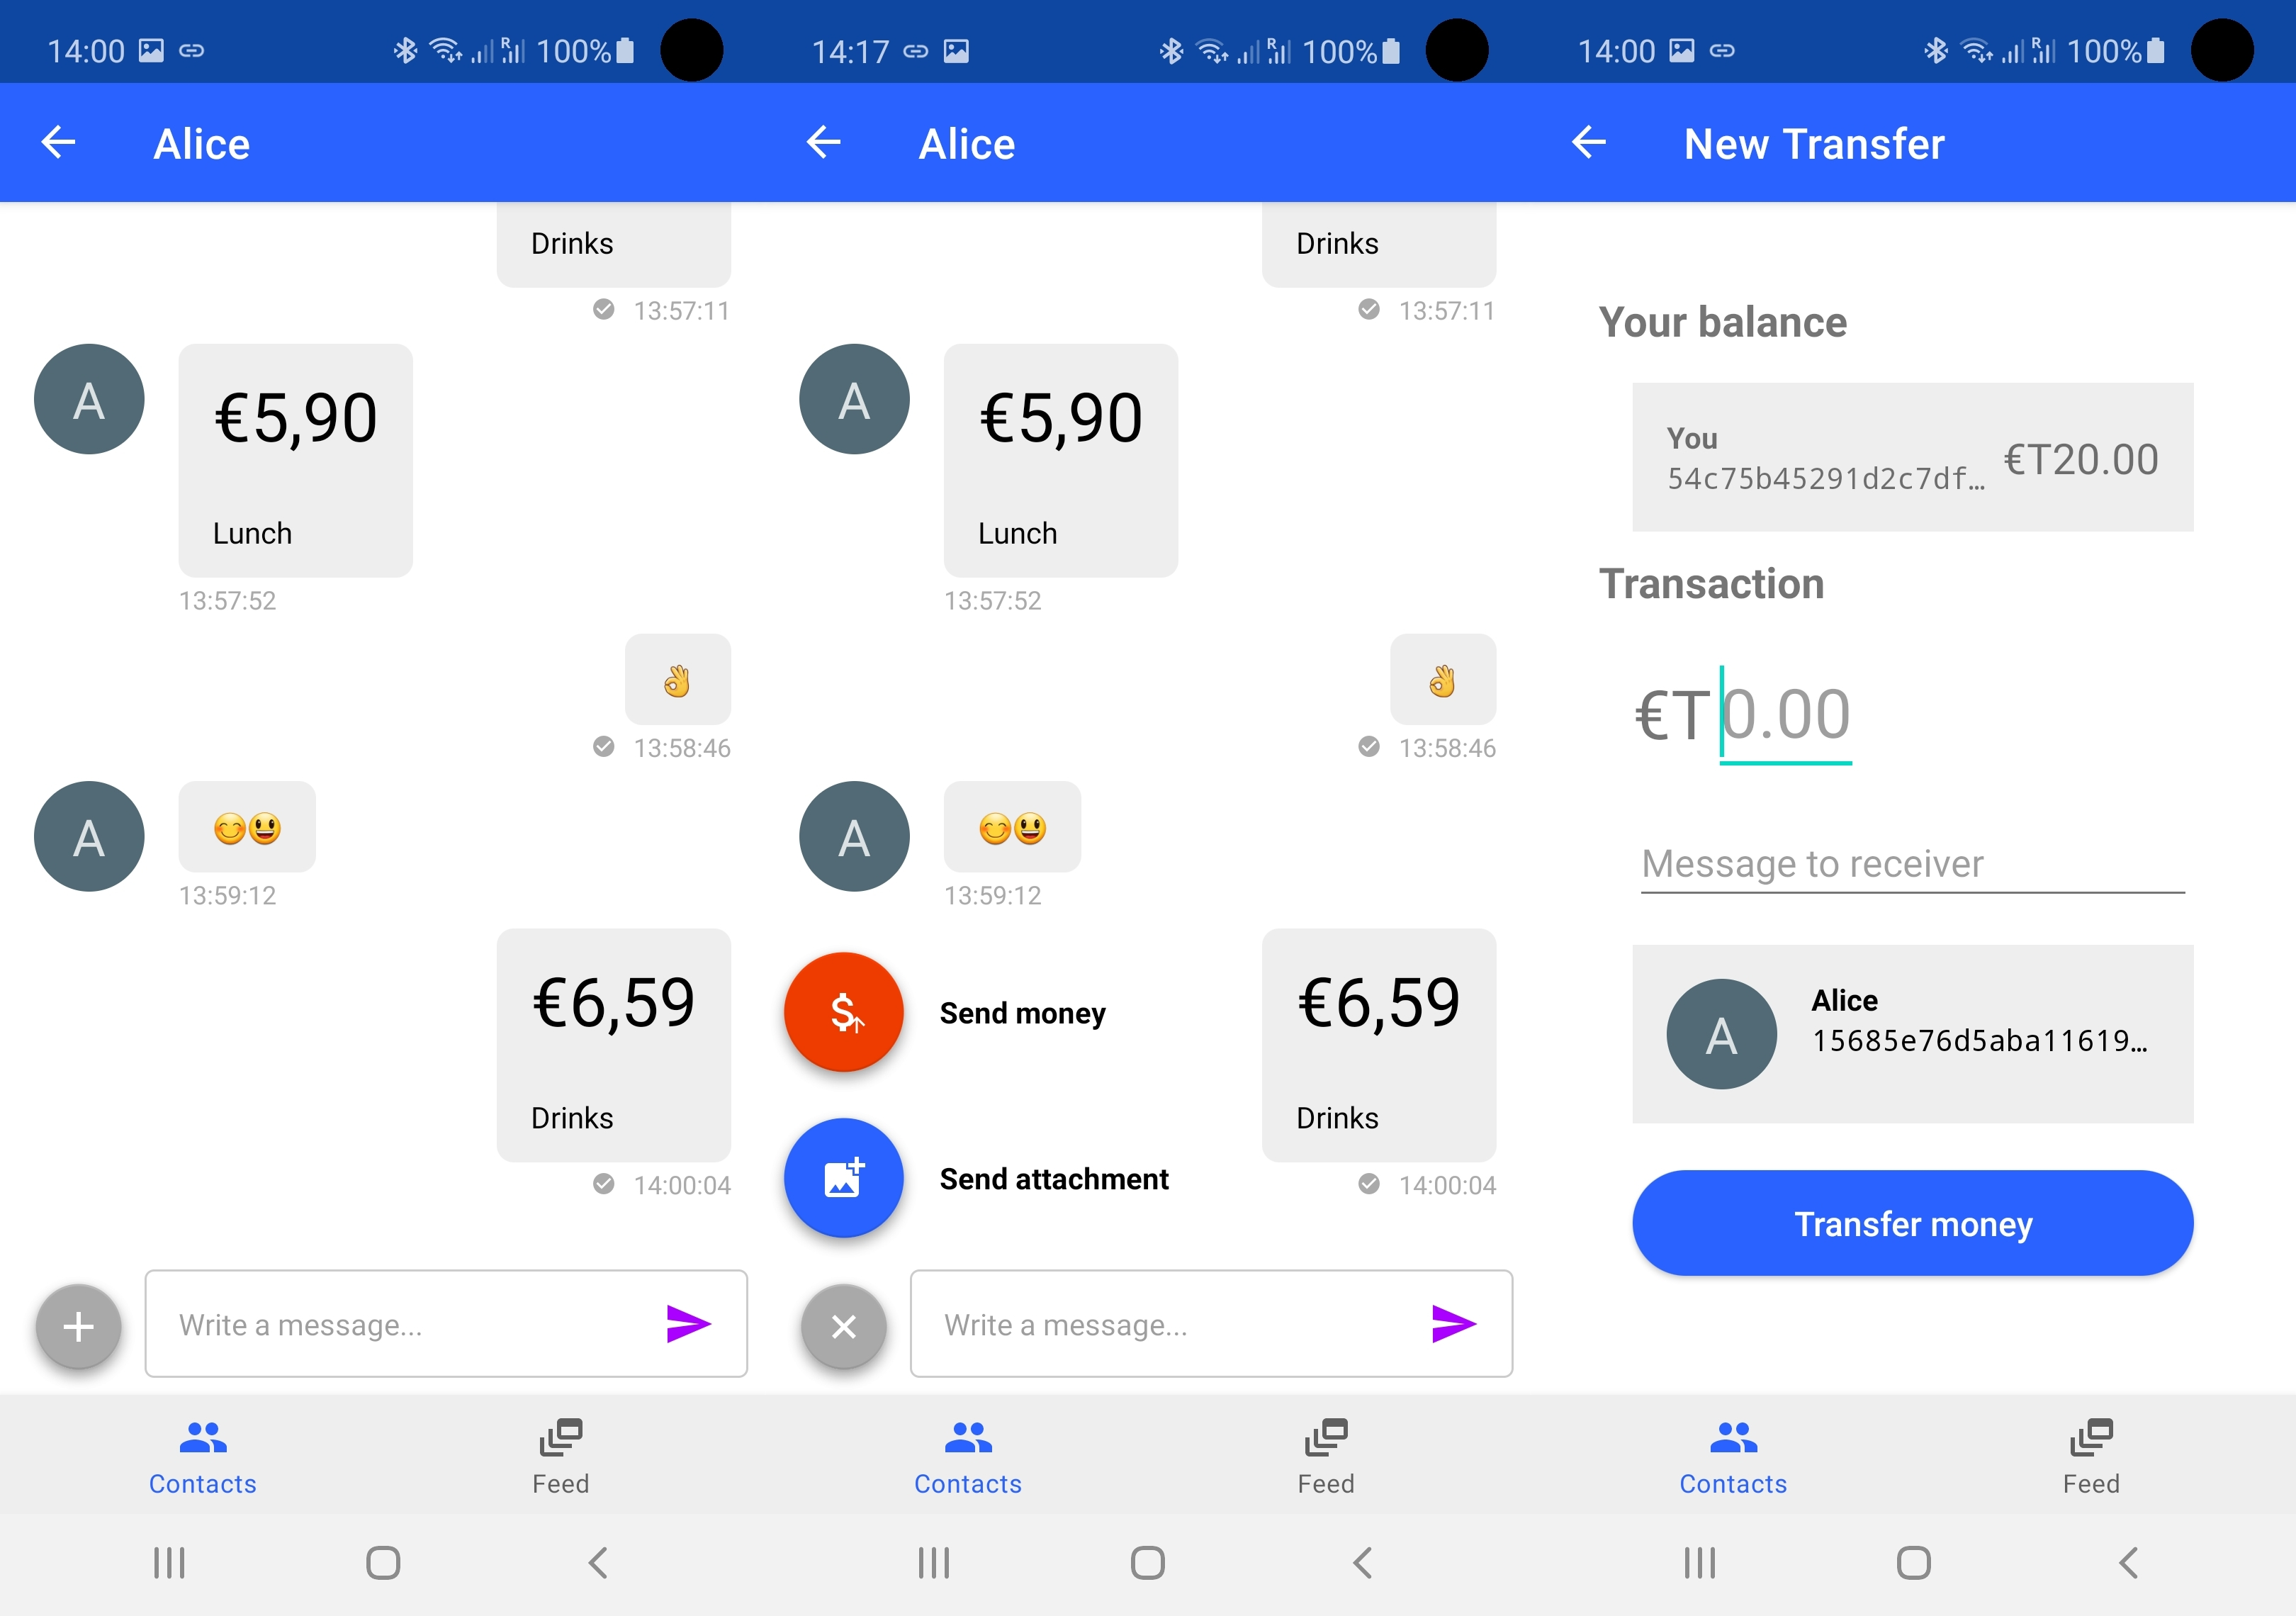
\includegraphics{../images/peerchat_send_money2.jpg}
\caption{Attach money in PeerChat \label{send_money_label}}
\end{figure}

The capacity to send transactions as shown in Figure
\ref{send_money_label} is not tied to PeerChat messaging. When money is
sent, a transaction is created and transferred to the receiver using the
TrustChain main community. The transaction hash is then sent as part of
the PeerChat message. The receiver then fetches the transaction it
received earlier via TrustChain.

\begin{itemize}
\tightlist
\item
  {[}TODO diagram of TrustChain and PeerChat interaction{]}
\end{itemize}

This implementation demonstrates the simple way in which EuroToken
allows monetary transactions to be seamlessly and programmatically
inserted into any application.

\subsection{EuroToken app}\label{eurotoken-app}

The PeerChat app is one specific use case. In reality different
applications would simultaneously use the EuroToken system. This would
leave the user with a splintered record of their financial life.

In order to solve this, a EuroToken accounting app has been added to the
super-app. The purpose of this is to show that the systems data can be
reorganized in whatever way. The EuroToken app shows a history of all
transactions, and provides another interface to the gateway.

\begin{figure}[htbp]
\centering
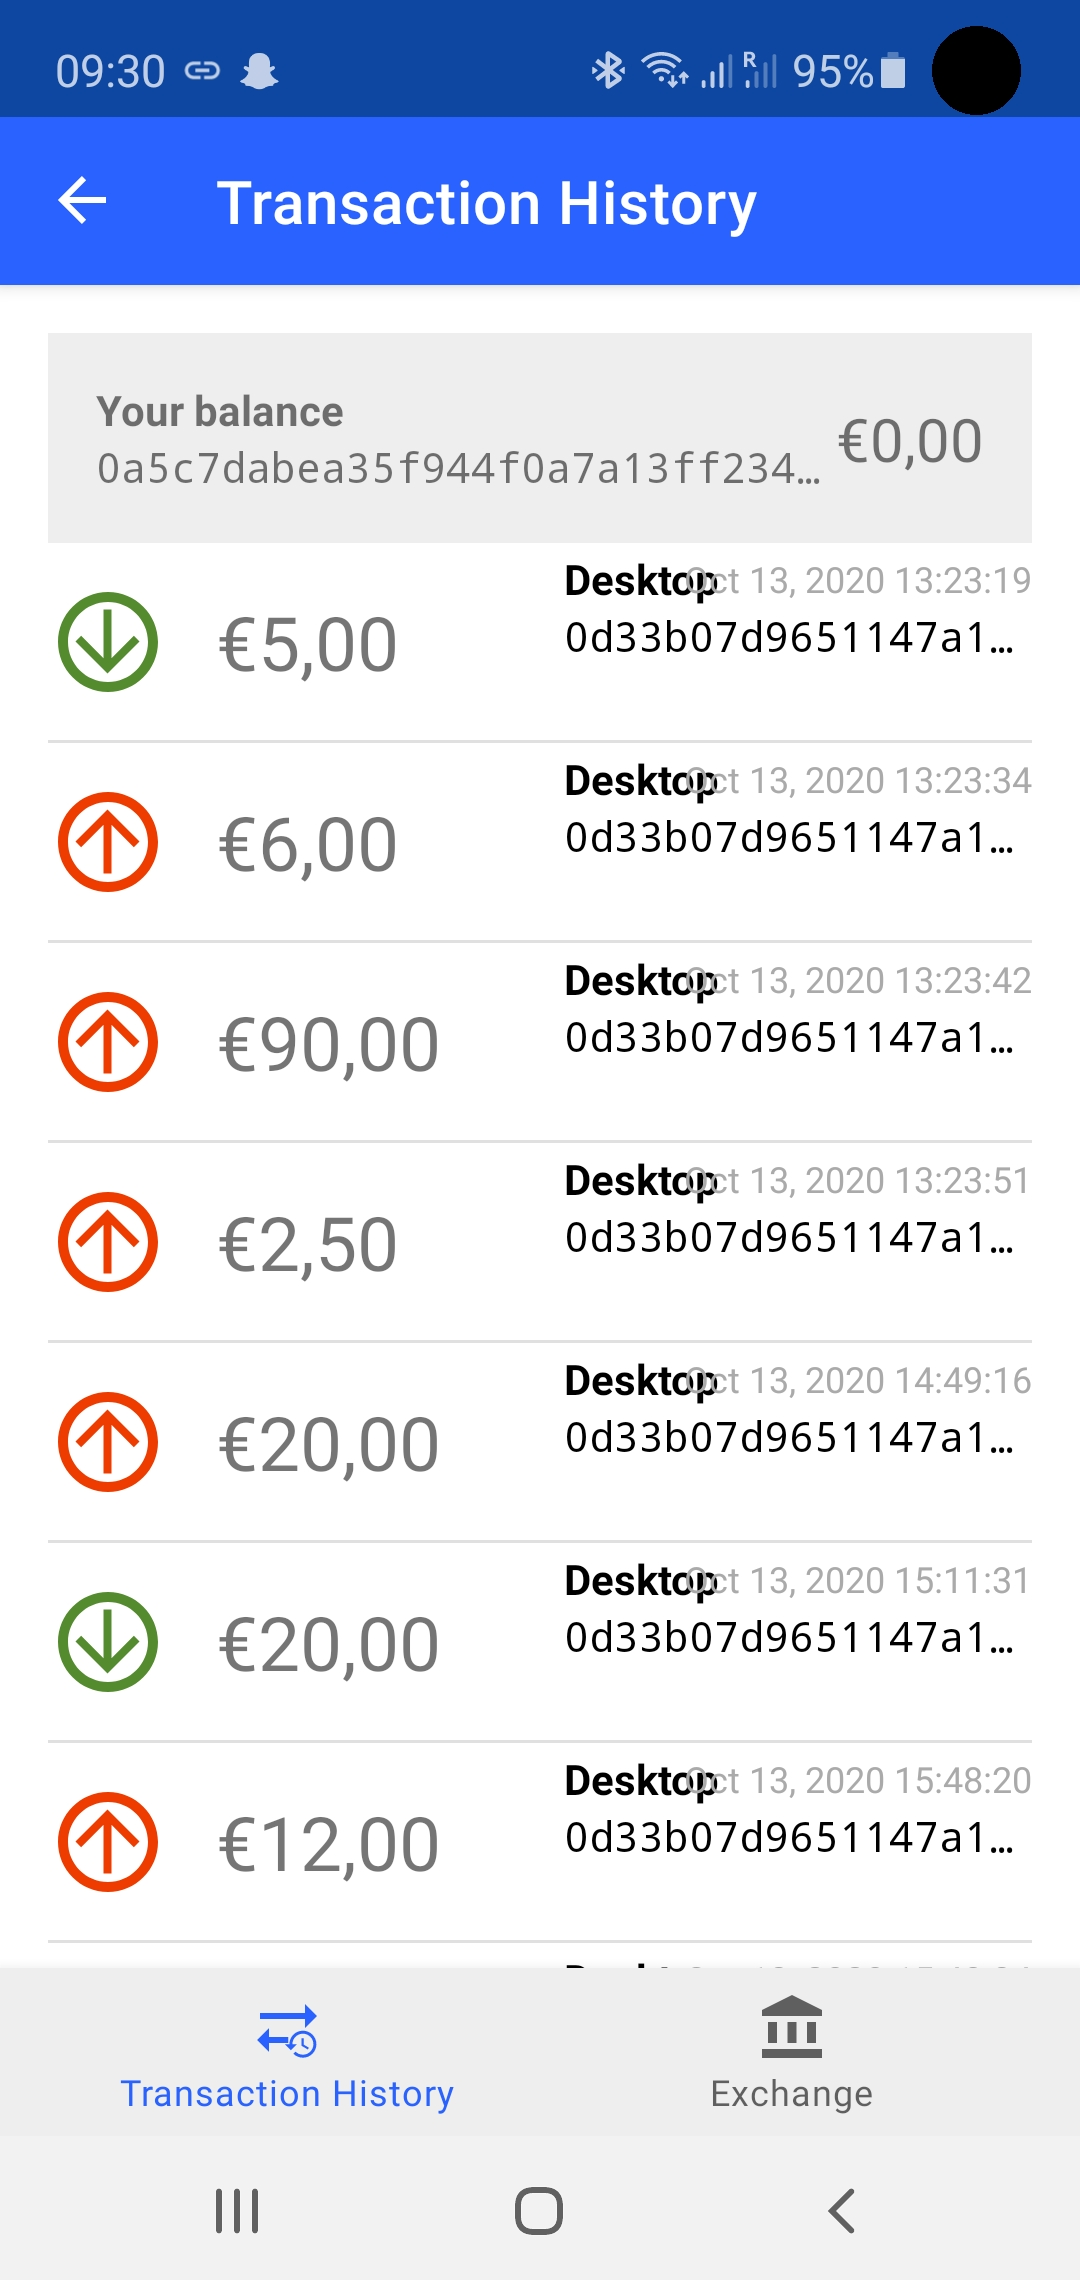
\includegraphics{../images/eurotoken_transaction_history.jpg}
\caption{EuroToken Transaction History
\label{transaction_history_label}}
\end{figure}

\subsection{EuroToken transactions in
depth}\label{eurotoken-transactions-in-depth}

\begin{itemize}
\tightlist
\item
  Validation (TODO)

  \begin{itemize}
  \tightlist
  \item
    Creation/destruction:

    \begin{itemize}
    \tightlist
    \item
      Trust Central Bank only
    \end{itemize}
  \item
    Transactions (prevent double spend)

    \begin{itemize}
    \tightlist
    \item
      Trusted users (based on identity later)
    \item
      Validated by bank
    \item
      Bami double-spend protection
    \end{itemize}
  \end{itemize}
\end{itemize}

\subsection{EuroToken Settings}\label{eurotoken-settings}

In addition to providing convenient services to the user, the EuroToken
app has some configuration options to give the user control over their
role in the EuroToken network.

\textbf{Trusted Minters} - Since the network has a central component
that regulates the creation and destruction of the tokens, a demo
requires a running server. Since there is no party to maintain such a
server indefinitely right now, an option is added to allow the user to
specify public keys of trusted ``central banks''. If this option is
enabled, the wallet in the super-app does only accepts blocks signed by
the configured public keys.

\begin{itemize}
\tightlist
\item
  {[}TODO: image of minter config{]}
\end{itemize}

\textbf{Trusted validators} - Validation of transactions and prevention
of double spending is unsolved in TrustChain but is an important part of
any currency. Solving this problem in general is being worked on {[}TODO
CITE bami{]} and is out of scope for this project. However the issue of
transaction finality being important to a EuroToken system, a way to
prevent double spending has been added. A transaction is not considered
final until a trusted entity has signed a block in the senders chain
that comes after the send block. This means that the trusted entity is
responsible for the validation of the block and its dependencies. These
validators can be configured in the app in order to make de demo
repeatable.

\begin{itemize}
\tightlist
\item
  {[}TODO: image of validator config{]}
\end{itemize}

\chapter{Field trial}\label{field-trial}

\chapter{Discussion}\label{discussion}

\section{System dangers}\label{system-dangers}

\subsection{Under-collateralization}\label{under-collateralization}

Causes:

\begin{itemize}
\tightlist
\item
  By central bank printing without collateral
\item
  Licenced gateway banks going bust, taking collateral with them
\end{itemize}

Effects:

Future bank runs could leave some token holders without their
collateral, this makes token holders less confident in tokens. This
would lower their value, but the direct exchange peg maintains the
price. This hides the problem while undermining trust in the value of
the tokens.

Solution:

\begin{itemize}
\tightlist
\item
  Don't print without collateral.
\item
  Short term:

  \begin{itemize}
  \tightlist
  \item
    Keep collateral liquid at all times (also stops inflation)
  \end{itemize}
\item
  long term:

  \begin{itemize}
  \tightlist
  \item
    see system future
  \end{itemize}
\end{itemize}

\section{System future}\label{system-future}

\begin{itemize}
\tightlist
\item
  euros are deleted by banks on euro2token exchange, and created on
  token2euro exchange.
\item
  Banks don't manange the collateral, only the CBDC exchange.
\item
  Banks get a place in trust instead of investment.
\end{itemize}

\chapter{Conclusion}\label{conclusion}

\chapter*{Related Work}\label{related-work}
\addcontentsline{toc}{chapter}{Related Work}

\hypertarget{refs}{}
\hypertarget{ref-ipv8}{}
Tribler. n.d. ``Tribler/Py-Ipv8: Python Implementation of the Ipv8
Layer.'' Accessed: June 13, 2020.
\url{https://github.com/Tribler/py-ipv8}.

%% Use letters for the chapter numbers of the appendices.
\appendix

%\input{appendix-a}

\nocite{*}

\bibliography{../bibliography.bib}

\end{document}

